\chapter{Componentes del Hardware}

\thispagestyle{plain}
\renewcommand{\tablename}{Tabla}

\section{Introducción}

Un vehículo robótico típicamente consta de varias partes esenciales que trabajan en conjunto para su funcionamiento. Se diferencian partes mecánicas y electrónicas. En el sistema mecánico podemos encontrar el chasis, que proporciona la estructura física sobre la cual se montan todos los componentes. Ya en el sistema electrónico encontramos: sensores, que permiten al vehículo percibir su entorno; actuadores, responsables de ejecutar acciones físicas como respuesta a señales recibidas; unidad de control, encargada del procesado de datos y toma de decisiones basadas en algoritmos; una fuente de energía, que permita alimentar el vehículo; y por último un sistema de comunicación, que facilite la interacción del vehículo con otros dispositivos.

En este capítulo se describirán los componentes principales del hardware que han sido utilizado en el desarrollo de este proyecto. Comentando sus características y el uso que se hace de los mismos. El enfoque principal estará en los componentes empleados para la comunicación, el control y el actuador.

\section{Motores sin escobillas}
En la actualidad, podemos diferenciar cinco tipos de motores en función del tipo de energía que utilizan, encontrando motores de gasolina, diésel, eléctricos, híbridos y de gas. Siendo la tendencia la utilización de motores eléctricos. Dentro de estos podemos encontrar varios tipos, aunque los más utilizados son los Paso a Paso, \textit{Brushed} y \textit{Brushless}. 

El motor eléctrico basa su funcionamiento en la capacidad de convertir energía eléctrica en energía cinética, y para este efecto se sirve de la energía magnética por la que se repelen dos campos. Los motores de corriente continua sin escobillas, \textit{Brushless Direct Current (BLDC)}, no emplean escobillas para el cambio de polaridad en el rotor. La ausencia de escobillas hace que tenga una vida útil mayor requiriendo bajo mantenimiento. Además, debido a la falta de fricción en el interior del motor hace que tenga una mayor potencia, velocidad y eficiencia, y que por la misma razón produzca un menor ruido. 

En este proyecto se utilizarán los servomotores BLDC GIM8108 V3 de SteadyWin (Figura \ref{fig:Motor-GIM8108v3}), caracterizados por ser motores de corriente continua sin escobillas que utilizan el protocolo de comunicación CAN bus. 

\begin{figure}[H]
    \centering
    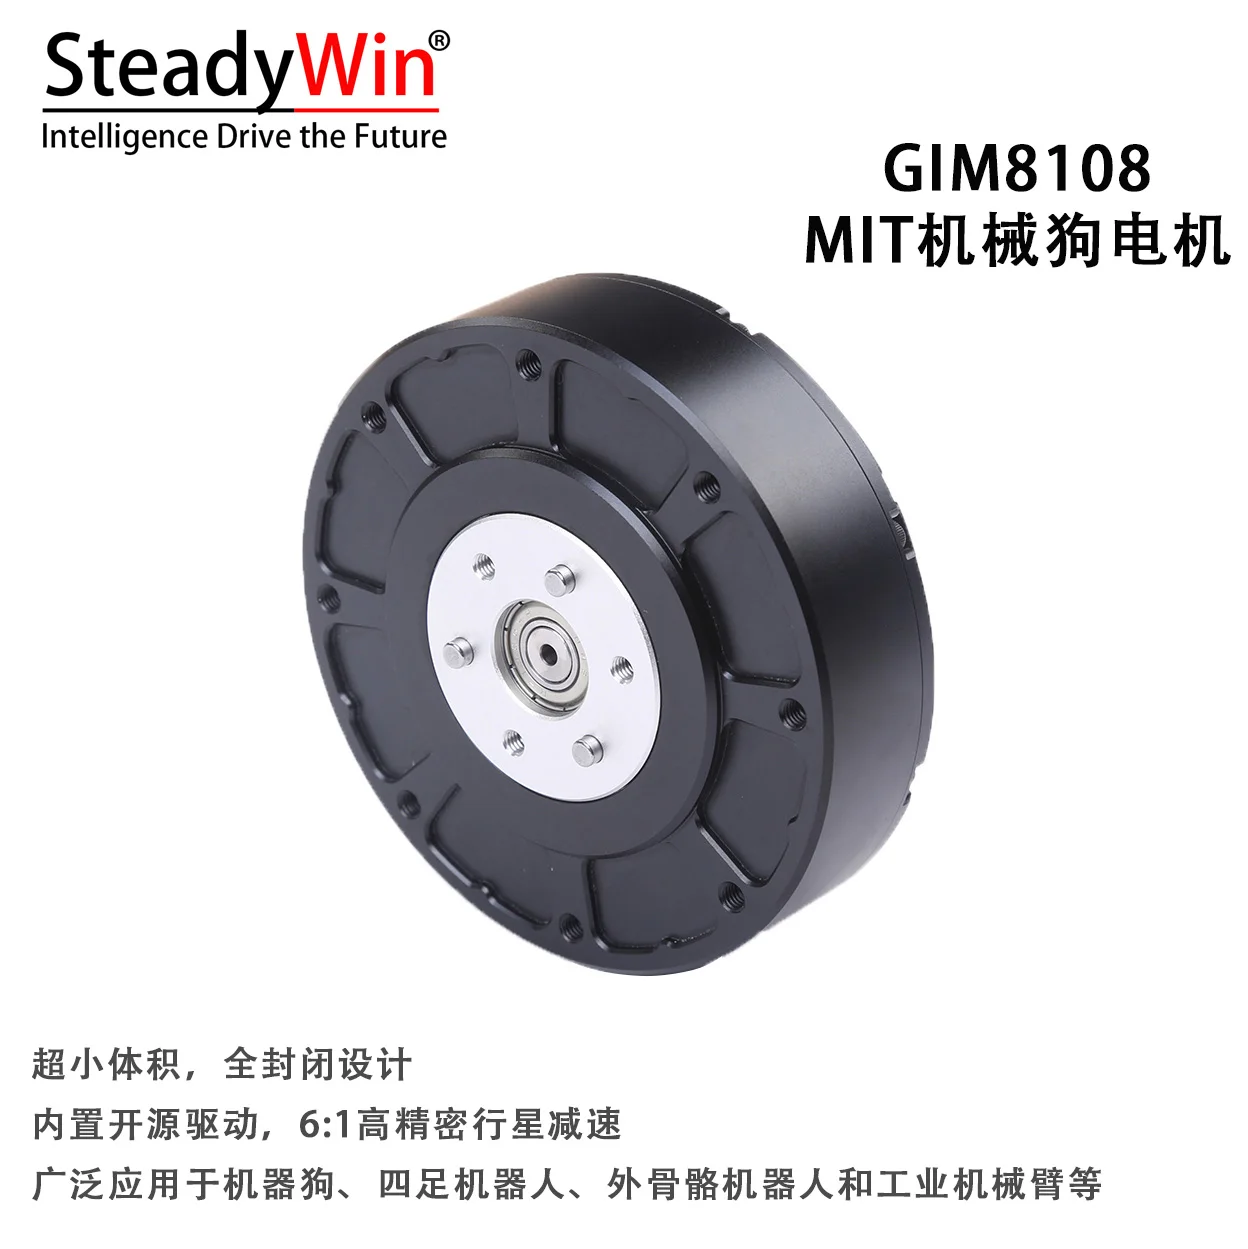
\includegraphics[width=0.75\linewidth]{imagenes/GIM8108.png}
    \caption{Motor GIM8108 v3 \cite{江西伺泰威自动化设备有限公司}}
    \label{fig:Motor-GIM8108v3}
\end{figure}

La falta de documentación por parte del fabricante dificultó el inicio del proyecto. A partir de uno de estos ficheros \cite{GIM8108v3} se obtiene los parámetros del motor.

\begin{table}[H]
    \centering
    \begin{tabular}{| l | l | p{5cm} |}
         \hline
         \rowcolor{lightgray}
         \multicolumn{3}{| c |}{\textbf{Parámetros del motor GIM8108v3}}\\
         \hline
         \multirow{2}{4em}{Alimentación} & Voltaje & \(24 VDC \pm 10 \%\)\\
         & Intensidad & \(7 A\) \\
         \hline
         \multirow{4}{4em}{Detalles} & Torque (par) & \(1,27 Nm\) \\
         & Velocidad de giro & \(1500 rpm\) \\
         & Velocidad máxima & \(2000 rpm\) \\
         & Potencia & \(200 W\) \\
         \hline
         \multicolumn{2}{|l|}{Señal de realimentación} & Encoder absoluto de \(15\) bits, un giro representa \(32768\)\\
         \hline
         \multicolumn{2}{|l|}{Relación de transmisión} & \(6:1\)\\
         \hline
         \multicolumn{2}{|l|}{Torque de parada en funcionamiento} & \(15 Nm\) \\
         \hline
         \multicolumn{2}{|l|}{Modo de refrigeración} & Refrigeración natural \\
         \hline
         \multicolumn{2}{|l|}{Peso} & \(600 g\) \\
         \hline
         Control de posición & Frecuencia de muestreo & \(2 kHz\) \\
         \hline
         \multicolumn{2}{|l|}{Protección} & Aviso de bloqueo del rotor \\
         \hline
         \multicolumn{2}{|l|}{Interfaz de comunicación} & Smartcan (CAN, \(1 MHz\) ) \\
         \hline
         \multirow{3}{4em}{Entorno de trabajo} & Temperatura ambiente & \(0-40 \degree C\) \\
         & Temperatura máxima permitida & \(85 \degree C\) \\
         & Humedad & \(5-95 \%\) \\ 
         \hline
    \end{tabular}
    \caption{Características del motor GIM8108 v3}
    \label{tab:my_label}
\end{table}

\section{Sistema Electrónico con Arduino Mega}

El siguiente esquema (Figura \ref{fig:Fritzing-ConexionArduinoMega}) se ha realizado con Fritzing. En su realización se ha seguido el código de colores empleado en el vehículo, a excepción de la señal CAN\_H, cuyo color gris apenas se diferenciaba del color blanco de la señal CAN\_L. Los motores GIM8108 utilizados en este proyecto no se encuentran modelados en Fritzing por lo que se representan mediante un conjunto Motor BLDC - Controlador de Potencia. Por último, las baterías y la \textit{shield} del Arduino, se han reemplazado por unas de iguales características pero de aspecto y marca distinta.

\begin{figure}[H]
    \centering
    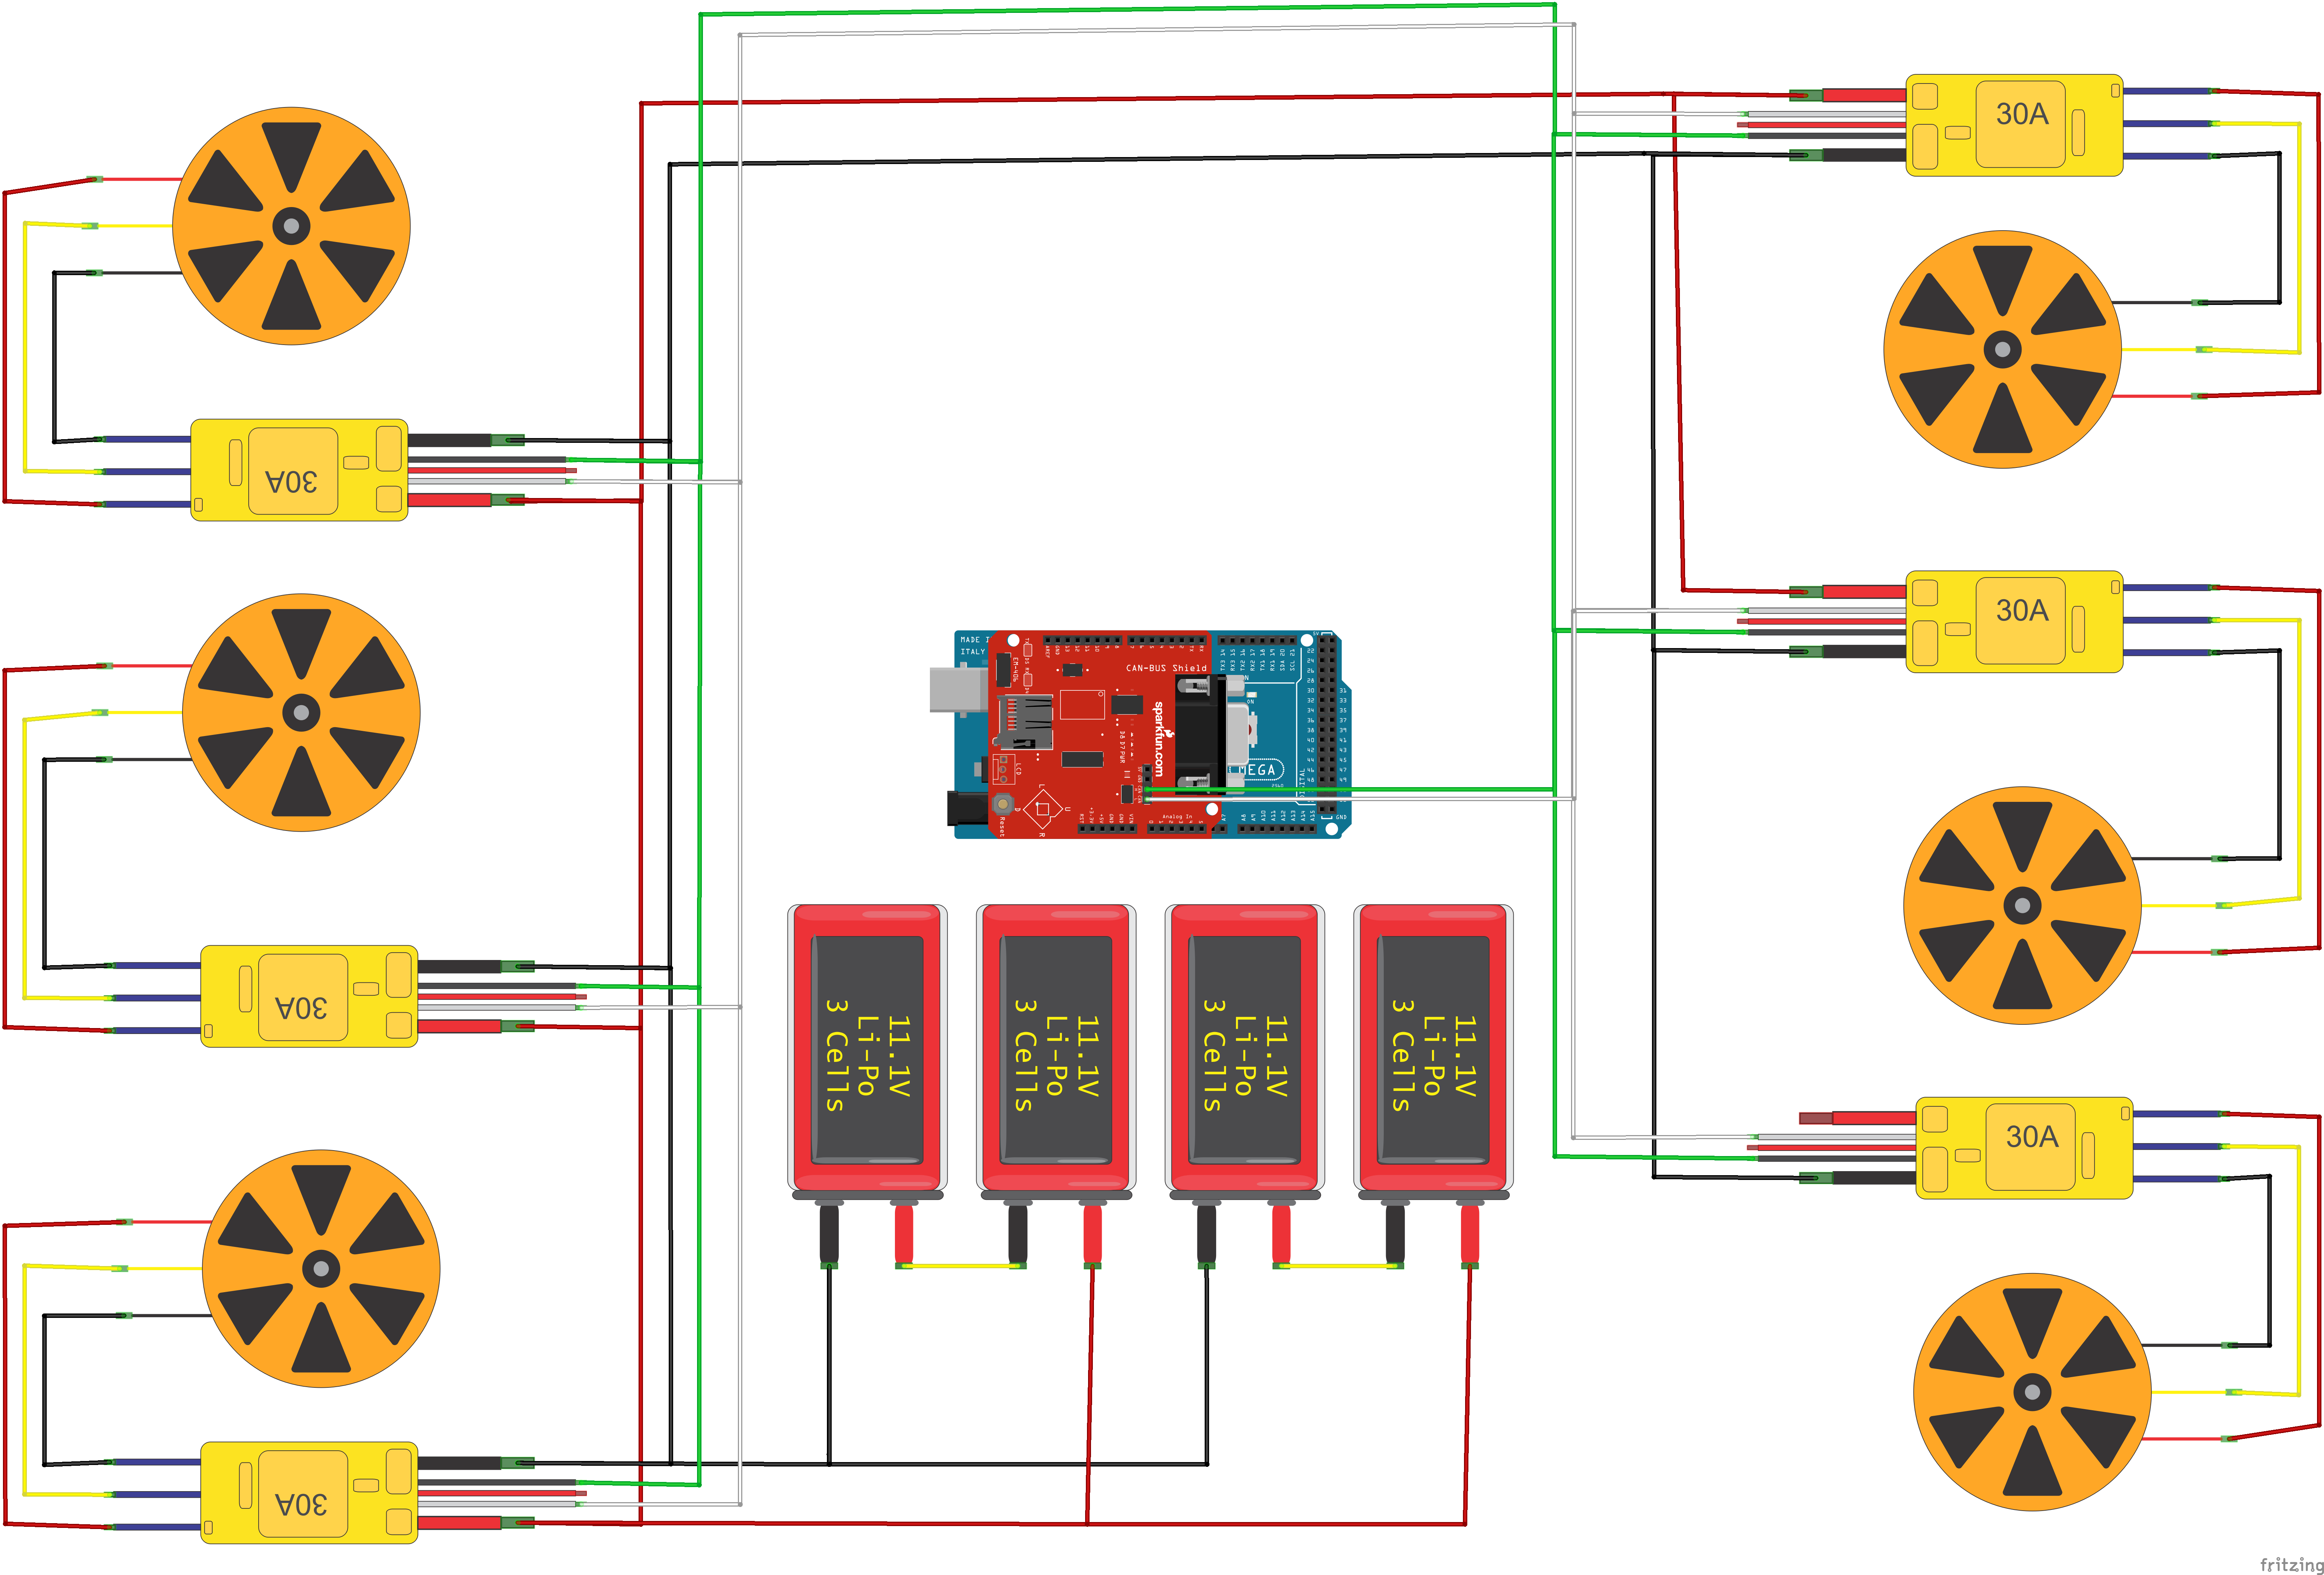
\includegraphics[width=1\linewidth]{imagenes/ConexionDonatello - ArduinoMega2560_bb.png}
    \caption{Esquema de conexiones del vehículo.}
    \label{fig:Fritzing-ConexionArduinoMega}
\end{figure}

\subsection{Arduino Mega 2560}

Esta placa es parte de la familia de placas Mega, las cuales destacan por su uso en proyectos que demandan mucha potencia informática. Además posee un mayor número de puertos de entrada/salida, interfaces e interrupciones que otras placas de la familia. Esto y su suporte en Simulink, es el motivo por el cuál se utiliza el Arduino Mega 2560 para este proyecto.

La placa Arduino Mega 2560 es una actualización que reemplaza a la placa Arduino Mega. Esta nueva placa está basada en el microcontrolador ATmega2560. Posee 54 pines de entrada/salida digitales (15 de ellos pueden ser utilizados para salidas de PWM), 16 entradas analógicas, 4 UARTS (puertos seriales), un cristal oscilador de 16 MHz, conector USB, puerto de alimentación, conector ICSP y botón de reset.

\begin{figure}[H]
    \centering
    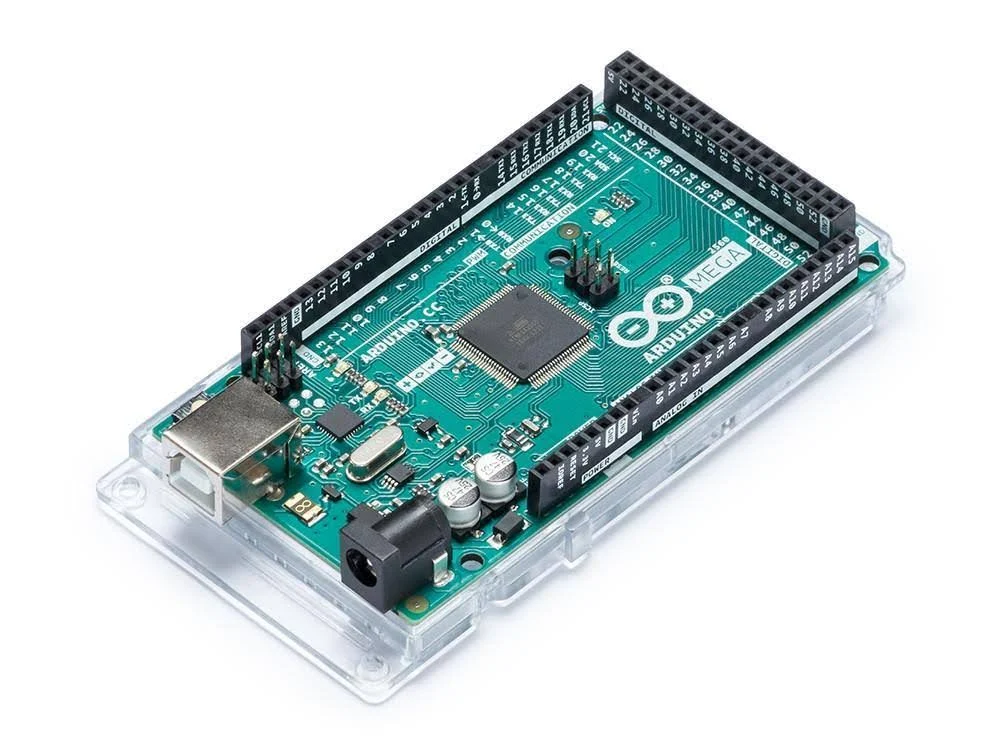
\includegraphics[width=0.5\linewidth]{imagenes/Arduino Mega 2560.png}
    \caption{Arduino Mega 2560 \cite{ArduinoMega2560rev3}}
    \label{fig:arduino-mega2560}
\end{figure}

\subsection{CAN-BUS Shield v1.2}

Esta \textit{shield} funciona perfectamente con las placas Arduino UNO (ATmega328), Arduino Mega (ATmega1280/2560) y Arduino Leonardo (ATmega32U4).

\begin{figure}[H]
    \centering
    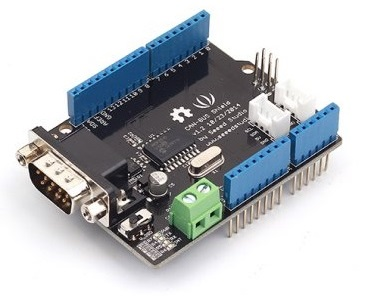
\includegraphics[width=0.5\linewidth]{imagenes/Arduino Mega CAN Shield.png}
    \caption{CAN-BUS Shield v1.2 \cite{ArduinoMegaCANShield}}
    \label{fig:Arduino-megaCANShield}
\end{figure}

Características:
\begin{itemize}
    \item Implementa CAN V2.0B hasta 1Mb/s
    \item Interfaz SPI hasta 10MHz
    \item Marcos de datos y remotos estándar (11 bits) y extendidos (29 bits)
    \item Dos búferes de recepción con almacenamiento de mensajes priorizados
    \item Conector sub-D de 9 pines estándar industrial
\end{itemize}

\begin{figure}[H]
    \centering
    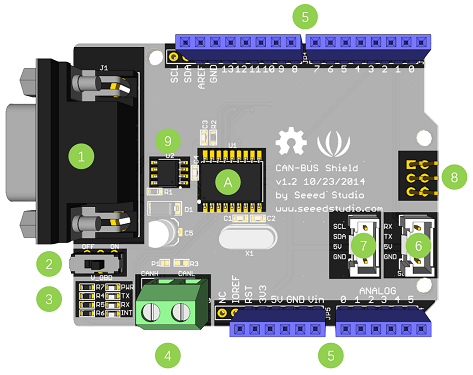
\includegraphics[width=0.5\linewidth]{imagenes/Arduino Mega CAN Shield PARTES.png}
    \caption{CAN-BUS Shield v1.2 \cite{ArduinoMegaCANShield} - Descripción General}
\end{figure}

Descripción General:

\begin{enumerate}
    \item Interfaz DB9: Para conectar a la interfaz OBDII a través de un cable DBG-OBD
    \item V\_OBD: Se alimenta de la interfaz OBDII (desde DB9)
    \item Indicador LED:
    \begin{itemize}
        \item PWR: Potencia
        \item TX: Parpadea cuando se envían datos
        \item RX: Parpadea cuando se reciben datos
        \item INT: Interrupción de datos
    \end{itemize}
    \item Terminal: CAN\_H y CAN\_L
    \item Pines de Arduino UNO
    \item Conector Serial Grove
    \item Conector I2C Grove
    \item Pines ICSP
    \item CI - MCP2551, un transceptor CAN de alta velocidad
    \item CI - MCP2515, controlador CAN independiente con interfaz SPI
\end{enumerate}

\section{Sistema Electrónico con Arduino MKR}

\subsection{Arduino MKR WiFi 1010}

Esta placa es parte de la familia de placas MKR, cada una de las cuales cuenta con un módulo de radio que facilita la comunicación a través de Wi-Fi, Bluetooth, LoRa, Sigfox y NB-IoT. Todas las placas de esta serie se fundamentan en el procesador de bajo consumo Arm Cortex-M0 de 32 bits SAMD21, y además incluyen un chip criptográfico para asegurar la comunicación de manera confiable.

La sustitución de la placa Arduino Mega 2560 por una Arduino MKR WiFi 1010 permitirá la incorporación de comunicaciones inalámbricas con el vehículo robótico. Además, se aumenta la velocidad del reloj de \(16\ MHz\) a \(48\ MHz\), lo que implica un incremento en la rapidez con la que la placa recupera e interpreta instrucciones. 

\begin{figure}[H]
    \centering
    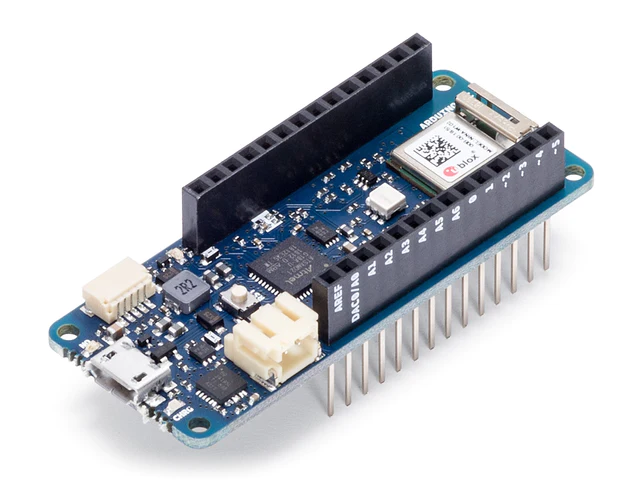
\includegraphics[width=0.5\linewidth]{imagenes/Arduino MKR WiFi 1010.png}
    \caption{Arduino MKR WiFi 1010 \cite{ArduinoMKRWiFi1010}}
    \label{fig:MKR-WiFi1010}
\end{figure}

Sus especificaciones técnicas son:

\begin{table}[H]
    \centering
    \begin{tabular}{|l|p{7cm}|}
        \hline
        \rowcolor{lightgray}
        \multicolumn{2}{|c|}{\textbf{Especificaciones técnicas}} \\
        \hline
        Microcontrolador & MCU ARM de bajo consumo SAMD1 Cortex-M0+ de 32 bits \\
        Módulo Radio & u-block NINA-W102 \\
        Alimentación & \(5 V\) \\
        Elemento Seguro & ATECC508 \\
        Batería Compatible & Li-Po Single Cell, 3.7V, 1024mAh Mínimo \\
        Voltaje de Operación del Circuito & \(3,3 V\) \\
        Pines E/S Digital & 8 \\
        Pines PWM & 13 \\
        UART & 1 \\
        SPI & 1 \\
        I2C & 1 \\
        Pines Entrada Analógica & 7 \\
        Pines Salida Analógica & 1 \\
        Interrupciones Externas & 10 \\
        Corriente Continua por Pin E/S & \(7 mA\) \\
        Memoria Flash CPU & \(256 KB\) \\
        SRAM & \(32 KB\) \\
        EEPROM & no \\
        Velocidad de Reloj & \(32,768 kHz\) (RTC), \(48 MHz\) \\
        LED Integrado & 6 \\
        USB & Dispositivo USB de alta velocidad y host integrado \\
        Largo & \(61,5 mm\) \\
        Ancho & \(25 mm\) \\
        Peso & \(32gr\) \\
        \hline
    \end{tabular}
    \caption{Especificaciones técnicas del Arduino MKR}
    \label{tab:MKR-Especificaciones}
\end{table}

\subsection{Arduino MKR CAN Shield}

La MKR CAN Shield simplifica la conexión de las placas MKR con sistemas industriales, especialmente con aplicaciones automovilísticas. Esta \textit{shield} añade posibles aplicaciones en vehículos inteligentes, coches autónomos y drones, al facilitar la conexión a través del protocolo CAN. Además, permite conectar directamente una placa MKR a diversos tipos de sensores, motores y pantallas industriales, brindando una solución versátil para una amplia gama de proyectos.

\begin{figure}[H]
    \centering
    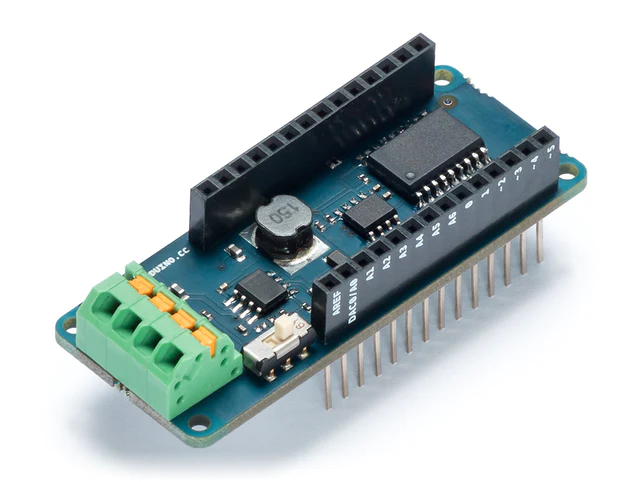
\includegraphics[width=0.5\linewidth]{imagenes/Arduino MKR CAN Shield.png}
    \caption{Arduino MKR CAN Shield \cite{ArduinoMKRCANShield}}
    \label{fig:MKR-CANShield}
\end{figure}

Sus especificaciones técnicas son:

\begin{table}[H]
    \centering
    \begin{tabular}{|l|l|}
        \hline
        \rowcolor{lightgray}
        \multicolumn{2}{|c|}{\textbf{Especificaciones técnicas}} \\
        \hline
        Protocolo & CAN Bus \\
        Interfaz & SPI \\
        Voltaje de funcionamiento del circuito & \(3,3 V\) \\
        Controlador & Microchip MCP2515 \\
        Transceptor & NXP TJA1049 \\
        Convertidor Buck & Texas Instruments TPS54232 \\
        Vin () & \(7V - 24V\) \\
        Vin () & \(5V\) \\
        Compatibilidad &  MKR \\
        \hline
    \end{tabular}
    \caption{Especificaciones técnicas del Arduino MKR Shield}
    \label{tab:MKRShield-Especificaciones}
\end{table}


\section{Chip MCP2515}

El MCP2515 del fabricante Microchip Technology es el controlador que encontramos en las \textit{shields} de Arduino utilizadas en este proyecto.Es un controlador CAN de segunda generación capaz de transmitir y recibir tanto tramas de datos estándar como extendidos a una velocidad máxima de \(1 Mb/s\) . Este microchip se comunica con microcontroladores a través de una Interfaz Periférica Serial (SPI) estándar en la industria.

\begin{figure}[H]
    \centering
    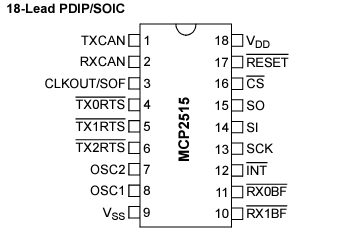
\includegraphics[width=0.75\linewidth]{imagenes/MCP2515.png}
    \caption{MCP2515 - Microchip Technology \cite{MCP2515}}
    \label{fig:MCP2515-chip}
\end{figure}

\subsection{\textit{SPI - Serial Peripheral Interface}}

La interfaz de periféricos en serie (SPI) es un bus de interfaz utilizado habitualmente para enviar datos entre microcontroladores y pequeños periféricos como registros de desplazamiento y sensores. Incluye una línea de reloj, dato entrante, dato saliente y un pin de selección, que se encargará de elegir el dispositivo con el que se va a establecer la comunicación.

\begin{figure}[H]
    \centering
    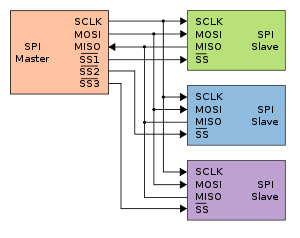
\includegraphics[width=0.75\linewidth]{imagenes/SPI.png}
    \caption{Conexión bus SPI \cite{Wiki-SPI}}
    \label{fig:SPI-Conexión}
\end{figure}

La principal diferencia entre este puerto serie y uno común se encuentra en la señal de reloj. Un puerto serie común, con líneas TX y RX, se conoce como ``asíncrono'' porque no hay control sobre cuándo se envían los datos ni ninguna garantía de que ambos lados estén funcionando a la misma velocidad. Dado que los ordenadores se basan normalmente en que todo está sincronizado con un único reloj, esto puede ser un problema cuando dos sistemas con relojes diferentes intentan comunicarse entre sí. SPI funciona con un bus de datos ``síncrono'', lo que significa que utiliza líneas separadas para los datos y un reloj que mantiene ambos lados en perfecta sincronía, sin necesidad de especificar la velocidad, aunque si se deberá tener en cuenta las velocidades máximas a la que pueden funcionar los dispositivos.



\subsection{\textit{CAN - Controller Area Network}}

El protocolo CAN Bus es un estándar de comunicación utilizado en sistemas electrónicos distribuidos. CAN es el acrónimo de \textit{Controller Area Network}, es decir, Red de Área de Controlador. En el ámbito de la informática hace referencia a un elemento que transmite una elevada cantidad de información.

Este protocolo fue desarrollado en la década de 1980 por la compañía alemana Bosch, inicialmente para su uso en automóviles, pero hoy en día su uso se ha extendido a diferentes sectores, incluyendo el industrial, el médico y el de servicios públicos.

\begin{figure}[H]
    \centering
    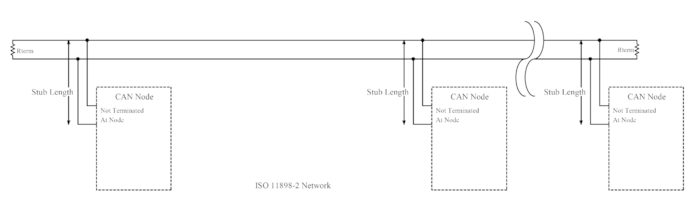
\includegraphics[width=\linewidth]{imagenes/CAN.png}
    \caption{Conexión bus CAN \cite{Wiki-CAN}}
    \label{fig:CAN-Conexión}
\end{figure}

Los mensajes se transmiten mediante un bus de datos compartido, lo que significa que todos los dispositivos conectados a la red pueden recibir el mensaje. Cada mensaje tiene una identificación única que sirve para distinguirlo de otros mensajes en la red.

\begin{figure}[H]
    \centering
    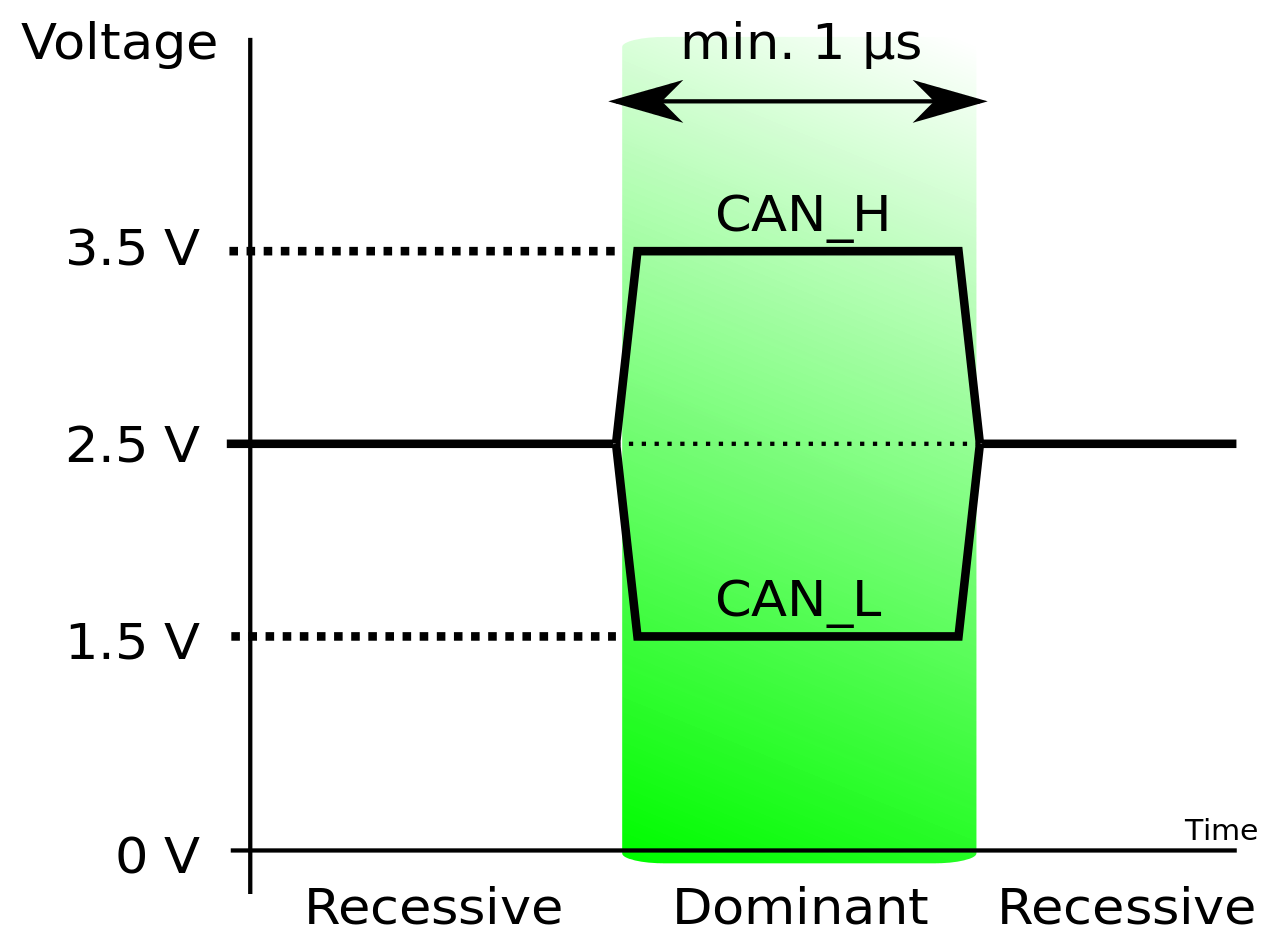
\includegraphics[width=0.5\linewidth]{imagenes/CAN1.png}
    \caption{Niveles de tensión del CAN Bus \cite{Wiki-CAN}}
    \label{fig:CAN-Tension}
\end{figure}

Para interconectar los distintos dispositivos solo son necesarios dos cables (CAN\_H y CAN\_L) y una resistencia de \(120 \Omega\). Dependiendo del voltaje de estas señales, el bus puede encontrarse en modo recesivo, donde ambos están al mismo nivel de tensión, o en modo dominante, en la que se encuentran con una diferencia de tensión mínima de \(1,5V\). La lectura de los bits se basa en esta diferencia de voltaje entre los cables, lo que proporciona una mayor protección frente a interferencias electromagnéticas.

%\blankpage